\documentclass{article}

% if you need to pass options to natbib, use, e.g.:
\PassOptionsToPackage{numbers, compress}{natbib}
% before loading neurips_2020

% ready for submission
% \usepackage{neurips_2020}

% to compile a preprint version, e.g., for submission to arXiv, add add the
% [preprint] option:
    \usepackage[final, nonatbib]{neurips_2020}

% to compile a camera-ready version, add the [final] option, e.g.:
 %    \usepackage[final]{neurips_2020}

% to avoid loading the natbib package, add option nonatbib:
%     \usepackage[nonatbib]{neurips_2020}

\usepackage[utf8]{inputenc} % allow utf-8 input
\usepackage[T1]{fontenc}    % use 8-bit T1 fonts
\usepackage{hyperref}       % hyperlinks
\usepackage{url}            % simple URL typesetting
\usepackage{booktabs}       % professional-quality tables
\usepackage{amsfonts}       % blackboard math symbols
\usepackage{nicefrac}       % compact symbols for 1/2, etc.
\usepackage{microtype}      % microtypography
\usepackage{subcaption}
\usepackage{graphicx}
\usepackage{multicol}
\usepackage{wrapfig}
\usepackage{amssymb}
\usepackage{amsmath}
\usepackage{siunitx} % Required for alignment
\usepackage{mathtools}
\usepackage{listings}
\usepackage{color}

\definecolor{dkgreen}{rgb}{0,0.6,0}
\definecolor{gray}{rgb}{0.5,0.5,0.5}
\definecolor{mauve}{rgb}{0.58,0,0.82}

\lstset{
  language=Python,
  aboveskip=3mm,
  belowskip=3mm,
  showstringspaces=false,
  columns=flexible,
  basicstyle={\small\ttfamily},
  numbers=none,
  numberstyle=\tiny\color{gray},
  keywordstyle=\color{blue},
  commentstyle=\color{dkgreen},
  stringstyle=\color{mauve},
  breaklines=true,
  breakatwhitespace=true,
  captionpos=b,
  tabsize=4
}

\DeclareMathOperator{\Lagr}{\mathcal{L}}
\DeclarePairedDelimiter{\ceil}{\lceil}{\rceil}

\usepackage[ 
	backend=bibtex8,     
    style=authoryear,	
    maxcitenames=2,      
    maxbibnames=25,  
    dashed = false,		
    hyperref=true,       
    bibencoding=inputenc,   
    useeditor=false,  
    uniquename=init,  
    doi=true,
    url=true,
    isbn = false,
    giveninits = true,
    natbib=true
]{biblatex}

\sisetup{
  round-mode          = places, % Rounds numbers
  round-precision     = 4, % to 4 places
}

\addbibresource{references.bib}

\title{Are transformer models in time series forecasting worth the hustle? \\
        \Large A data driven Approach}
        
\author{Jan Besler \\
        5629079}

\begin{document}

\maketitle

\tableofcontents

\lstlistoflistings

\newpage

\section{Introduction}

\subsection{To-Do}

\begin{itemize}
   \item anhand von Korrdinaten gucken wo genau welche turbine steht, map basteln und average wind einzeichnen
   \item Graphen eFormer aktualisieren
   \item Colab einrichten \& Jobs starten
   \item Informer und Autoformer auf selbe Daten trainieren
   \item Auswertung vorbereiten
   \begin{itemize}
       \item Tabelle für Ressourcen Effizienz
       \item Vergleich Modelle zu Ground Truth -> 1 bis 3 Monate
       \item Comparison of Errors -> Werte mit Softmax angleichen?!
   \end{itemize}
   \item Related Work schreiben
   \item alle Formeln haben gleich Variablen Namen
\end{itemize}

\subsection{Motivation}

In early 2023, Large Language Models (LLM) attracted much public attention with the emergence of ChatGPT. The development of these models can be traced back to the development of transformer models, which have proven useful in the field of NLP. These transformer models use sequential data as input, i.e. a data point depends on the previous data points.
These Transformer models are also popular in other fields, such as time series forecasting, where the data is sequential by definition. In this research area, other models still receive a lot of attention, for example Long Short Term Memory (LSTM). The question therefore arises why Transformer models are not solely used for time series forecasting? This question was investigated by \cite{transformers-effectiveness} and their hypothesis is that it depends on the complexity of the underlying data which model performs better.
They concluded that transformers only have an advantage when they work with complex data structures, such as languages and text data. Thus, a transformer model with less complex data may lead to worse results compared to another model such as an LSTM. \par 
In order to investigate the hypothesis put forward by \cite{transformers-effectiveness}, this thesis will test different models on data with different levels of complexity. The data chosen is from wind turbines for the more complex side and electricity consumption from different companies on the less complex side. These applications were chosen to investigate how predictive models can be improved. And whether it is generally worthwhile to develop more complex models for different use cases if they might give worse results than previous solutions. \par 

In the area of electricity generation and consumption, forecasting is a relevant issue to drive the decarbonisation of the economy through the deployment of renewable energy. With the introduction of more renewable energy systems, electricity production fluctuates more than before, while demand patterns remain largely the same. This leads to conflicts, as demand and production need to be perfectly matched at all times. In addition, the stability of the power grid must be taken into account, as a production peak can lead to problems with the frequency of the power grid, which in turn can lead to system-wide failures and power outages. To avoid these problems, it is important to predict electricity production with high accuracy in order to know when the flow of electricity needs to be regulated by the relevant authorities and companies. On the other hand, it is beneficial for companies to know when they will consume the amount of energy for the corresponding time. This makes it easier to plan ahead, to take advantage of lower prices on the spot market and is another contribution to the stability of the electricity grid.\par 

The deep learning models used, are probabilistic and not deterministic. This is due to the advantages of probabilistic models when working with noisy data and the resulting probability distributions as outcomes instead of deterministic values. With the ability to quantify the uncertainty of forecasts, there is an advantage to modelling in a probabilistic way by understanding the range and probability of possible outcomes. Even if there is no exact value for the outcome, ranges can be given to estimate how big the impact will be.
However, the disadvantages of working with probabilistic models are the increased complexity due to working with probability distributions as outcomes, making the results less intuitive to interpret. In addition, the increased complexity leads to higher computational costs and thus greater demands on limited resources.

The critical importance of time series forecasting in the advancement of renewable energy systems underscores the need for effective predictive models. The advent of Large Language Models (LLMs) such as ChatGPT in early 2023 has reignited interest in the underlying transformer models, whose sequential data processing capabilities have shown promise beyond the confines of Natural Language Processing (NLP). Despite their success, the adoption of transformer models in domains like time series forecasting, where data is inherently sequential, is not ubiquitous, presenting a research opportunity to investigate their relative efficacy compared to established models such as Long Short Term Memory (LSTM) networks.

Zeng et al., 2022 posited that the complexity of the data dictates the performance superiority between these models, a hypothesis that is both compelling and critical for applications where precision forecasting is pivotal. This thesis aims to explore this hypothesis by comparing the performance of different models on datasets with varying complexity levels, specifically focusing on wind turbine data for complex scenarios and electricity consumption for less complex cases. These domains have been strategically selected for their acute relevance to energy management and the pursuit of decarbonization.

The imperative to match electricity demand with the fluctuating supply from renewable sources, and the need for grid stability, establish a real-world urgency for this research. Probabilistic deep learning models offer a means to address these challenges, with their advantages in managing noisy data and providing forecasts with quantified uncertainties. This thesis will also scrutinize the trade-offs presented by probabilistic models, such as increased computational costs and the nuanced interpretation of their probabilistic outcomes. Through this analysis, the research endeavors to contribute to the optimization of energy systems and to the broader understanding of the applicability of advanced predictive models in strategic decision-making.

\subsection{Research Question}

This study aims to critically assess the value added by transformer models in time series forecasting by examining their accuracy, complexity, and resource demands in comparison to less complex models such as LSTMs. The research will seek to determine whether the benefits provided by transformers justify their implementation in practical applications where time and resources are significant constraints. Consequently, the central research question is articulated as follows: "To what extent do transformer models in time series forecasting provide a justifiable advantage over traditional methods considering their complexity and resource consumption?"

To address this multifaceted question, the research will be guided by a series of sub-questions:

\begin{enumerate}
    \item What constitutes an effective model in time series forecasting, balancing accuracy, training duration, interpretability, and resource utilization?
    \item How can we ensure comparability between different datasets to validate the results, accounting for variations in time intervals, time zones, data integrity, and relevance of external factors such as weather conditions?
    \item Under what circumstances do transformer models excel over linear and LSTM models, and what is the magnitude of improvement observed?
    \item Among the various transformer models analyzed, which demonstrates superior performance, and what are the distinguishing architectural features that contribute to this performance?
\end{enumerate}

Through this structured inquiry, the thesis will contribute to a nuanced understanding of the applicability and efficacy of transformer models in the field of time series forecasting.

\section{Related Work}

With the rise of the transformer models, in different applications as NLP and Computer Vision, so came the specialisations of these models as shown in \cite{Transformer-Survey}. These ideas of different approaches and goals also reached the time series models, several sub categories emerged as shown by \cite{Transformer-TS-Survey}, but one area of special interest for this paper is time series forecasting, where \cite{forecasting-overview} gives an overview of forecasting methods in the area of electricity production and consumption. A more specific overview of deep learning models in time series forecasting is done by \cite{Transformer-TS-PV}, even though it focuses on predicting data in the area of photovoltaic, the overview and explanations for energy related data is useful in this paper too and gives an overview for the models that are suitable. \par 
In the area of probabilistic forecasting the work by \cite{Prob-Forecast-Overview} shows the increasing interest in prediction intervals and densities, especially after the GEFCOM14 competition numerous papers on the issue of probabilistic forecasting have been published. After this surge, a few papers of interest for this paper have been published, these include the Informer model, utilising sparse attention mechanism by \cite{Informer}, the autoformer which emphasizes auto regression, written by \cite{autoformer}. The time2vec paper by \cite{time2vec} investigates how embeddings and positional encodings can differ for time series forecasting due to their periodic time features.

\section{Data}

Two data sets are used to compare the data complexity types. On the more complex side is SCADA wind farm data from \cite{Windpark_Data_1}, which is 10-minute SCADA and event data from the 6 Senvion MM92s at the Kelmarsh wind farm, grouped by year from 2016 to mid-2021. On the less complex side is electricity consumption data from 3 manufacturing companies in Germany provided by Fraunhofer IPA. The data is available in 15-minute intervals and shows the electricity consumption in a hierarchical representation.
Do determine the complexity of a data set, the auto correlation is being used as a metric. The lower the auto correlation the higher the data complexity. 

\subsection{Wind farms}

The two Windmill parks are located on the British Isle, the first park 'Kelmarsh' is located between Cambridge and Birmingham, while the second park is located south-east of Edinburgh on the coast. 
Table \ref{tab:preprocessing_windturbines} shows a summary of some pre-processing steps conlcuded with the two data sets. A striking fact is the number of outliers in the \textit{Kelmarsh} Park, as well one Z-Score in the \textit{Penmanshiel} Park which indicates a electricity production of
\begin{equation*}
    \text{electricity production} = \mu + 497 \cdot \sigma
\end{equation*}
hence this is being dropped for being a technical mistake, since the wind speed at that time did not change compared to the hours before and after. 

\begin{table}[!ht]
\small
\centering
    \begin{tabular}{l|c|r|r|r|S|r}
    \toprule
    \textbf{Location} & \textbf{Turbine} & \textbf{Total Values} & \textbf{Missing Values} & \textbf{Outliers} & \textbf{Highest Z-Score} & \textbf{Stationarity} \\
    \midrule
\textbf{Kelmarsh} & 1 & 288 864 & 3449 & 6 & 3.835573 & yes \\
         & 2 & 288 864 & 3041 & 5 & 3.636474 & yes \\
         & 3 & 288 864 & 4195 & 3179 & 4.069864 & yes \\
         & 4 & 288 864 & 4938 & 2 & 3.370353 & yes \\
         & 5 & 288 864 & 3937 & 3091 & 4.793479 & yes \\
         & 6 & 288 864 & 5072 & 4625 & 5.445566 & yes \\
    \midrule
\textbf{Penmanshiel} & 01 & 266 435 & 1418 & 0 & 0.000000 & yes \\
            & 02 & 266 923 & 2903 & 1 & 3.441052 & yes \\
            & 04 & 265 447 & 924 & 1 & 3.374390 & yes \\
            & 05 & 265 135 & 802 & 1 & 3.479419 & yes \\
            & 06 & 267 012 & 3732 & 1 & 497.073209 & yes \\
            & 07 & 267 014 & 1032 & 1 & 3.595320 & yes \\
            & 08 & 259 106 & 3977 & 1 & 3.302787 & yes \\
            & 09 & 263 882 & 9076 & 0 & 0.000000 & yes \\
            & 10 & 263 412 & 8492 & 1 & 3.760396 & yes \\
            & 11 & 260 294 & 4977 & 1 & 3.372419 & yes \\
            & 12 & 262 702 & 7259 & 1 & 3.230310 & yes \\
            & 13 & 263 000 & 7841 & 0 & 0.000000 & yes \\
            & 14 & 261 694 & 7005 & 1 & 3.029291 & yes \\
            & 15 & 260 952 & 5640 & 1 & 3.298785 & yes \\
    \bottomrule
    \end{tabular}
\caption{Summary of Pre-processing Steps for Wind Turbine Data}
\label{tab:preprocessing_windturbines}
\end{table}

To investigate when the missing values occurred the power generation has been mapped in figure \ref{fig:Kelmarsh-missing-values} over the whole time span while the missing values have been color coded in red.
\begin{figure}
    \centering
    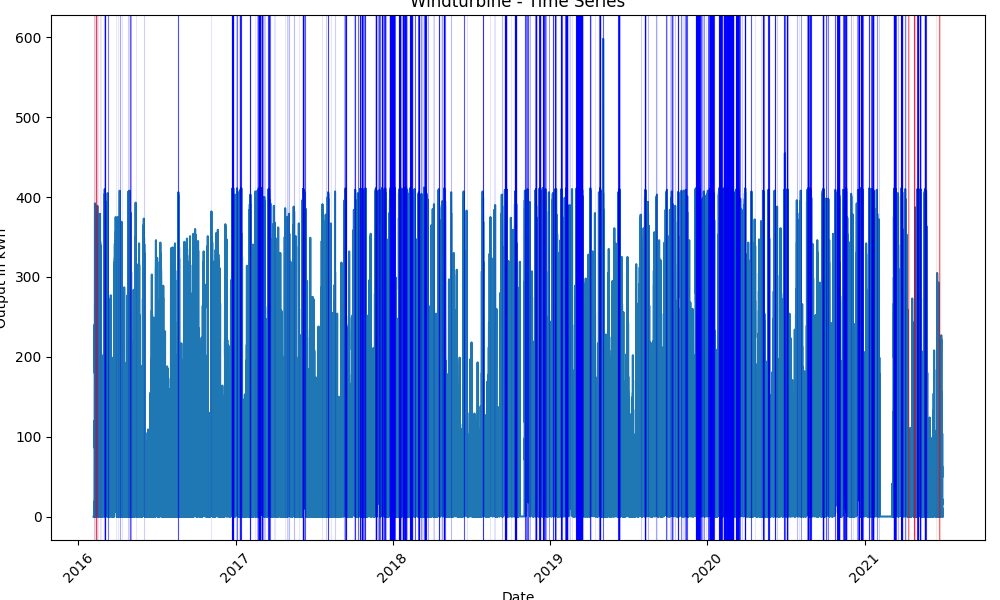
\includegraphics[width=\linewidth]{graphs/Windturbine - Time Series.png}
    \caption{Complete Power Output - Kelmarsh \#6}
    \label{fig:Kelmarsh-missing-values}
\end{figure}

Here it becomes visible that most of the missing values are all found in the beginning of the time series, this could be an indicator that not every wind mill was being monitored from the same time on wards as different magnitudes in the missing values for the different turbines show. As a result all missing values in the beginning are being dropped as well as all sequences in each time series with a duration of more than 3 hours since keeping these values does not hold any value for the forecasting task. These outages could be attributed to for example maintenance work. Sin

For the already mentioned problem of having too many outliers in 3 of 6 turbines remains. Outliers in this context have been defined as
\begin{equation}
    |\text{outlier}| >= 3 * \left( \frac{x - \mu}{\sigma} \right)
\end{equation}
the factor of three was chosen instead of the more usual two to account for extremes in wind speed especially in the coastal areas. To visualize the potential outliers all values for the Kelmarsh Wind park have been mapped as a kernel density estimation. The left figure \ref{fig:Kelmarsh-distribution} shows that the majority of values are centred around zero, hence no electricity output and presumably no wind speed. But there is also the practice of turning a turbine out of the wind if the situation demands it, hence no electricity production even though there would be enough wind. To test this hypothesis an deeper analysis of the turbine 6 was done to investigate how often this particular turbine was turned out of the wind. This was defined as 
\begin{equation}
    \text{out of wind} = \text{Wind speed (m/s)} > 3 \land \text{Power (kW)} < 1 
\end{equation}
resulting in $8705$ values being flagged, or equally $3.16 \%$ of all values. Therefor the data is being removed since the decision of turning a turbine out of the wind is influenced more by the stock exchange prices or the load factor of the electricity grid and has nothing to do with the prediction based on weather indicators. \par 
The extent can also be seen in the visualization of the $6^th$ turbine in the right figure \ref{fig:Kelmarsh-distribution}

\begin{figure}[h!]
    \centering
    \begin{subfigure}[b]{0.45\linewidth}
        \centering
        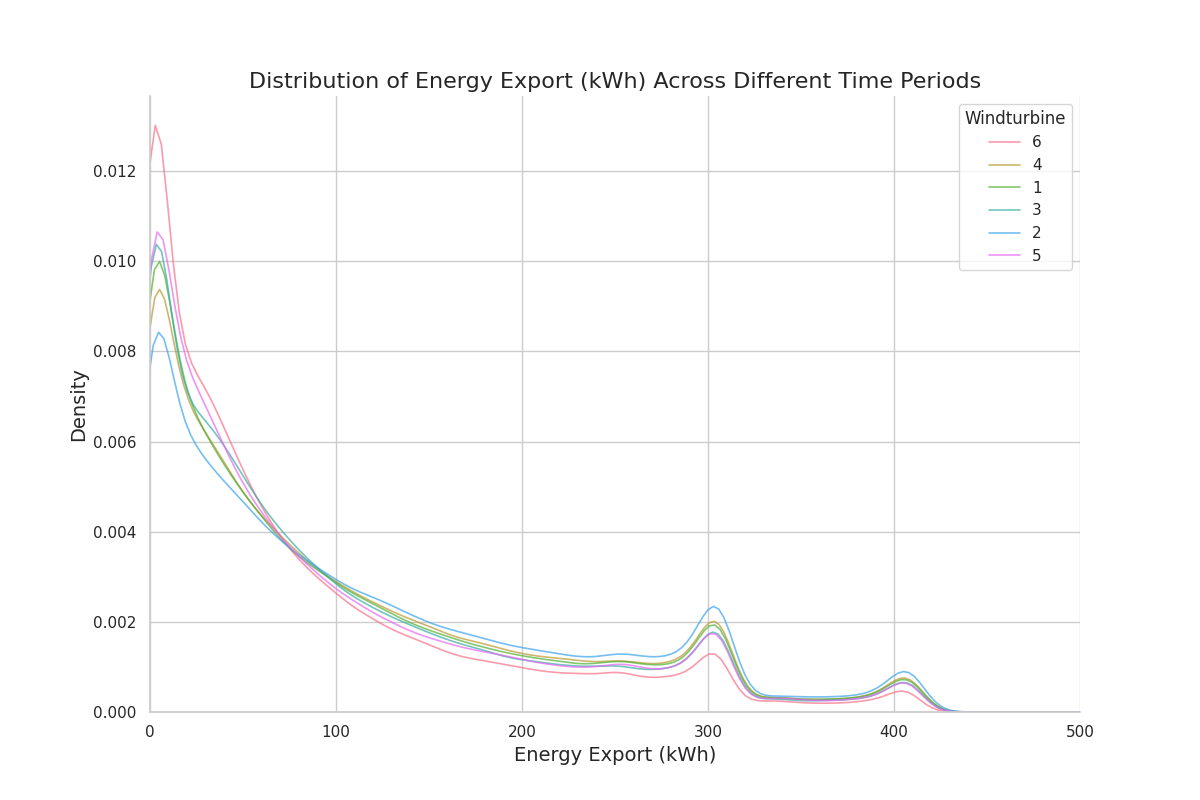
\includegraphics[width=\linewidth]{graphs/Kelmarsh_output_distribution.png}
        \caption{total}
    \end{subfigure}
    \begin{subfigure}[b]{0.45\linewidth}
        \centering
        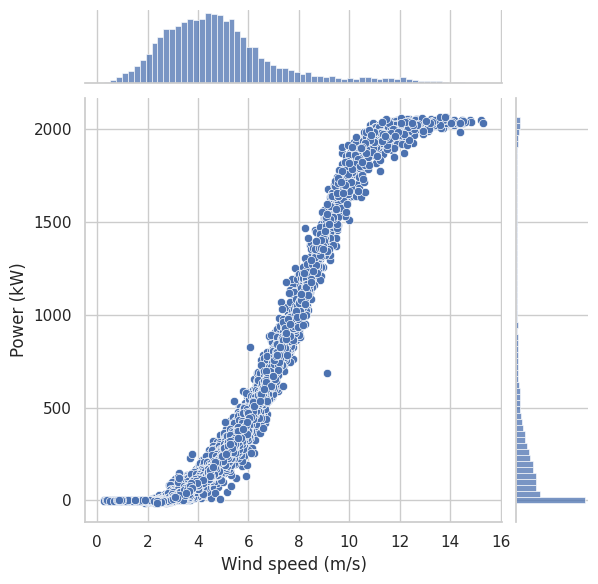
\includegraphics[width=\linewidth]{graphs/Corr_Wind_Power.png}
        \caption{\#6}
    \end{subfigure}
    \caption{Kelmarsh power distribution}
    \label{fig:Kelmarsh-distribution}
\end{figure}





\subsection{Industrial Electricity Consumption}






\section{Methodology}

The models selected for evaluation are several different transformer models, an LSTM model and a non-machine learning based model that serves as a benchmark for the other models. For the benchmark task, the Random Forest was chosen because of its numerous applications in the field of time series forecasting in previous work. The models that use deep neural networks are not written from scratch, but come from various publicly available libraries (PyTorch). These basic models are then fine-tuned using hyperparameter search. For the transformer models, various models from renowned papers as well as a self-made shallow transformer are selected to test whether the depth of the network has a large impact on the results. The forecast horizons are 1 hour, 24 hours and 96 hours, with the last forecast being the most difficult task. This last number was chosen because the weather forecasts are also produced for a 96-hour period. This rating is based on the total computational time to evaluate all models and the computational resources in terms of GPU/CPU and RAM usage.\par 

It is difficult to quantify whether a model provides a benefit in terms of increased predictive accuracy compared to the computational costs spent on development. Due to scalability, a small increase in accuracy can justify huge development costs when deployed at scale. The data is first pre-processed in a data pipeline to detect outliers and find missing values that could later affect the models. In a second step, the data is fed into the different models, and each of the datasets is compared against certain metrics to measure the performance of the models. Finally, the results are printed in tabular form and presented graphically for better comparability in the paper. \par 
Though an important question remains, how to assess the goodness of the models in a more qualitative way. Is accuracy more important, than training time and resources or is a intuitive interpretation for a broader audience also important?

The aim for the newly developed model is generalization with complex and less complex data, therefor it is not planned to include layers for extra steps found in other models such as seasonal decomposition or trend analysis.

\subsection{Model Evaluation}
\subsubsection{Error Metrics}

To determine whether a Model is successful in their task, standardised methods of comparison are needed. These already exist for the accuracy, as the metric to determine the goodness of a model is measured in how small the error of a model is. These errors can be measured in different ways, with the most prominent ones in regression analysis being:

The Mean Absolute Error (MAE) is a widely used metric for evaluating the performance of regression models. It is defined as the average of the absolute differences between the predicted and actual values. Mathematically, it is expressed as:

\begin{equation}
\text{MAE} = \frac{1}{n} \sum_{i=1}^{n} \left| y_i - \hat{y}_i \right|
\end{equation}

where \(y_i\) and \(\hat{y}_i\) are the actual and predicted values, respectively, and \(n\) is the number of observations. MAE is easy to interpret and provides a linear penalty for each unit of difference between the predicted and actual values \cite{MAE_RMSE}.
Mean Absolute Percentage Error (MAPE) is another metric commonly used for evaluating regression models, particularly when the data spans several orders of magnitude. It is defined as:

\begin{equation}
\text{MAPE} = \frac{100}{n} \sum_{i=1}^{n} \left| \frac{y_i - \hat{y}_i}{y_i} \right|
\end{equation}

MAPE expresses the error as a percentage, making it unitless and easier to compare across different scales \cite{MAPE}.
Mean Squared Error (MSE) is a metric that measures the average of the squares of the errors between the predicted and actual values. It is defined as:

\begin{equation}
\text{MSE} = \frac{1}{n} \sum_{i=1}^{n} (y_i - \hat{y}_i)^2
\end{equation}

MSE penalizes larger errors more severely than smaller ones, making it sensitive to outliers \cite{MSE}.
Root Mean Squared Error (RMSE) is the square root of MSE and is defined as:

\begin{equation}
\text{RMSE} = \sqrt{\text{MSE}}
\end{equation}

RMSE has the same units as the dependent variable and is particularly useful when large errors are undesirable \cite{MAE_RMSE}.\par 

The previously introduced error metrics are not developed to handle probabilistic forecasts, unlike the Continuous Ranked Probability Score (CRPS) developed by \cite{Loss_Function} which is perfectly suited for probabilistic forecasts. This metric is especially suited for the evaluation since for a deterministic forecast, the metric becomes the MAE. Thus deterministic and probabilistic models can be evaluated using the same metric. Further this metric can also be used as a loss function, for the transformer models as a replacement for the usual cross entropy loss, since it has been used for probabilistic weather forecasts in several papers as \cite{CRPS_example_1, CRPS_example_2, CRPS_example_3} show. \par 
It is defined as:
\begin{equation}
    CRPS(F, x) = \int_{-\infty}^{\infty} ( F(y) - \mathcal{H}(y-x) )^{2} dy
\end{equation}
where $F$ is a cumulative distribution function of $X$, for example $F(y) = \mathbf{P}[X \leq y]$ with $x$ being the observation and $F$ is associated with an empirical distribution forecast. $\mathcal{H}$ is a step function along the real line that attains
\begin{equation}
    \mathcal{H} = \begin{cases}
        1, & \mathbb{R} \geq 0 \\
        0, & \text{otherwise}
    \end{cases}
\end{equation}

\subsubsection{Ressource Efficiency}

Utilizing each of these error metrics a wider range of potential problems and areas of interest (like the penalising of outliers) can be covered. But what is scarcely being looked upon are other metrics of evaluating models besides the accuracy, this includes resource efficiency and computational requirements linked to that the time to train and an intuitive interpretation of the results. In this thesis, these measurements are playing a bigger role in evaluating models besides the accuracy. Especially resource efficiency is playing a bigger role as shown by \cite{AI_energy_consumption} and \cite{resource_awareness}. One of the problems lies in size and complexity of machine learning models which alongside the volume of data required for the training have been experiencing exponential growth, thereby demanding more computational resources. This trend has outpaced the advancements in computing hardware platforms, storage infrastructure, and networking capabilities, leading to sustainability challenges. Some papers such as \cite{Informer} have implemented some aspects to reduce the computational efficiency, but their idea was more about training time than resource efficiency. \par 
The problem with evaluating the resource efficiency, is the lack of a proper framework and standardised measurements. It is not in the scope if this thesis to develop such frameworks, but to map the resources used to train different models on the same data and further the time spend during the whole development process on training, testing and performing inference on cloud computers is mapped, evaluated and critically viewed for improvements and saving opportunities. In order to achieve this goal, a function is running during the training, testing and evaluation process to map the CPU, RAM and GPU usage as well as the time it takes to train the model. These values are measured every 5 seconds, although this takes away resources from the models itself, the function is applied to all models and therefore the reduced capacity cancels out. In the end the values of interest are the average and peak usage to determine which models use are most cost efficient in terms of computational power used.

\subsection{Linear Models}

The linear model used in this thesis is nothing new, but is regarded as a benchmark towards the other models. To compare the more complex models to a very simple model, with the expectation that the more complex models outperform the simpler models. If that is not going to be the case or they achieve similar results, than the models are regarded as failures and are being discarded. \par 

The linear model is based on the same starting conditions as the other models, the same lags, the same variables in a multivariate context and the same data for the train, validation and test sections. What is not being included is a layer for seasonal decomposition as well as trend cycles, since the aim is to develop models can perform reasonable well without these to increase their generalization performance. This linear Model is a Single-Layer-Perceptron as \cite{transformers-effectiveness} have used as well in their work. This holds the advantage of producing weights which can be used in the weighted mean CRPS loss function, which is used as part of the different runs as well.
\begin{lstlisting}[language=Python, caption=Single-Layer-Perceptron]
class LinearModel(nn.Module):
    def __init__(self, input_size, output_size):
        super(LinearModel, self).__init__()
        self.linear = nn.Linear(input_size, output_size)

    def forward(self, x):
        x = self.linear(x)
        weights = self.linear.weight.data
        
        return x, weights
\end{lstlisting}\label{code:LinearModel}
The model consists of a single linear layer to keep this as simple as possible and achieving similar results to a linear ordinary least square regression. This model is expected to train the fastest and the least amount of resources compared to the deep learning models. Since the model works with the same batches from the data loader as the other models, the training process can be parallelised which helps with the speed of the training process. 


\subsection{Machine Learning Models}


\subsection{DeepLearning Models}

The goal in this section is to create a distinct Transformer model for time series forecasting, not from scratch but to dissect several different published models and evaluate what each of these models did differently and if the innovative parts is beneficial to this context and data. To get an understanding of the models one has to first in what regard each one differentiates from the vanilla model and also why and how they did it. \par 
Since the DeepLearning Models are in the centre of the research a thorough valuation of the performance of these models is conducted. With the different architectures different strategies to solve the same problem are being introduced. Therefor the results of all transformer models are compared separately in more depth, to investigate which of the architectures and strategies achieve the best performance. 

\subsubsection{Vanilla Transformer}

The vanilla transformer represents a version that is close to the original model presented by \cite{vanilla-transformer} that utilises the attention mechanism and is not optimised in any way to a time series forecasting role, hence it has no additional layers to perform seasonal decomposition or other methods.
The vanilla transformer has a standard encoder-decoder structure and uses fully connected layers, hence it is expected to use the most resources as no alterations have been undertaken to lower the complexity of its calculations. 

\subsubsection{Informer}

The Informer is a model developed by \cite{Informer} that sets itself apart by enabling multivariate instead of univariate probabilistic time series forecasting. The most distinct noticeable changes are the reduction of the computational requirements to calculate the attention mechanism and reduces the memory usage of the encoder/decoder layers. The first improvement refers to the complexity of calculation for the self-attention in the vanilla model, this can be described with the formula
\begin{equation*}
    O(T^2 \cdot D)
\end{equation*}
where $T$ is the length of the time series and $D$ is the dimension of the hidden states. The problem here lies in $T^2$ which explodes in the case of long sequences. Therefore the authors have proposed a different method called \textit{ProbSparse} that calculates the complexity of the self-attention calculation as
\begin{equation*}
    O(T \cdot log{T}) .
\end{equation*}
The idea is the differentiation between 'active' and 'lazy' parts where respective dot products contribute in different magnitudes towards the attention mechanism. The 'lazy' parts with a negligible contribution are left out and only the 'active' parts are considered
\begin{quote}
    Quadratic computation of canonical self-attention:
    The vanilla Transformer has a computational complexity of  where TT is the time series length and DD is the dimension of the hidden states. For long sequence time-series forecasting (also known as the LSTF problem), this might be really computationally expensive. To solve this problem, Informer employs a new self-attention mechanism called ProbSparse attention, which has time and space complexity.
    
    Memory bottleneck when stacking layers:
    When stacking NN encoder/decoder layers, the vanilla Transformer has a memory usage of , which limits the model's capacity for long sequences. Informer uses a Distilling operation, for reducing the input size between layers into its half slice. By doing so, it reduces the whole memory usage to be.
\end{quote}
Another interesting aspect that this paper utilises is the use of \textit{Probabilistic Time Embedding}. This method does not only encodes the data to vectors, but does also take into account the uncertainties associated with the given time information. This is particularly useful in contexts where the time variable plays a crucial role and its varying effect can not be mapped in a deterministic way. The idea behind this is that an embedding for a particular time step is not fixed but can be a distribution. Therefore, multiple possible embeddings could represent a single time step, capturing the inherent uncertainty or variability at that time. Hence a distribution in this context shows a set of possible vectors that could represent the embedding of a particular time series, instead of being listed as a single vector. Each vector sampled from this distribution would be a valid representation of the time series, allowing the model to capture the uncertainty associated with it. The reason why this can be useful in the context of Time Series Forecasting is due to the fact that the state of the system could be uncertain or subject to external factors not included in the model. In this cas, using a distribution over embeddings can help the model account for the corresponding uncertainty during training and inference.

\subsubsection{Autoformer}

\cite{autoformer}

\subsection{eFormer}

The eFormer is going to be the core of this analysis, it targets to be a domain specific probabilistic transformer model that outperforms more general models like the previously introduced Informer and Autoformer models. Even though the main performance measurement is going to be the accuracy of the forecast, another relevant metric to evaluate this model is the training time and resource consumption. Since this model is aimed to be as lightweight as possible. This should be achieved by dropping the entire decoder part and only use a minimal amount of layers and fewer heads than comparable models. While not writing new layers or parts, this paper uses already published parts from papers and searches for the optimal composition and combination to achieve the set goals. \par
The model architecture consists of the time2vec embeddings created by \cite{time2vec} with the positional encoding introduced by \cite{vanilla-transformer}, an auto-correlation mechanism by \cite{autoformer} that replaces the attention mechanism in a vanilla transformer and a sparse-attention mechanism that reduces the complexity calculation published by \cite{Informer}. The two attention modules are not used in a row after one another, but parallel where each odd and even back propagation loop runs on a different attention class. This is due to the inner workings of both attention mechanisms, since both filter out irrelevant parts and with too much filtering more information is lost than initially desired and the weights are converging towards zero too fast, leaving fewer non-zero elements in the weights than desired. Hence in the first step there are going to be four models, only one attention mechanism per model and each mechanism as a probabilistic and a deterministic variant. The probabilistic model introduces uncertainty in the very beginning and carries the respective Gaussian distributions based on the mean and the variance trough all the way, thus being computationally more expensive but with the potential of keeping more information since the variance is trained independently from the mean in case they are not correlated. The other case, what is referred to as deterministic model, only learns the mean of the distributions and the variance is only inferred after the training is completed in a separate probabilistic layer where the uncertainty is introduced to give a hint on how accurate the estimates are. Though this is a computationally cheaper option is does not provide the same degree of information regarding the uncertainty of the predictions, hence this is a less desirable variant. \par 
The model utilises the early stopping technique to have the potential of saving resources and avoid unnecessary training time if the loss does not change significantly anymore. 

\subsubsection{Data Loader}

The data loader is used to prepare the input data sets by ensuring they have the right dimensions and to prepare the batches which are later fed into the transformer model. Thus it enables parallelization and also the last steps of data engineering. At first the data is shifted $n$ time stamps which are determined in the hyperparameters by the variable \textit{look\_back} resulting in a data frame of shape $(\text{dependent variable}(look\_back + 1) + \text{independent variable}(look\_back), \text{time stamps})$, hence each row in this new data frame acts as one observation where the first value is the ground truth and the other values are lagged values of the dependent and independent variables. The dependent variables for the same time stamp as the true value have been omitted, since would enable the model to work with data from the future. After shifting the data, the data frame is split into a train, test and evaluation data set, this process includes shuffling since each row is its own time series with little connections to the other time series. If the data is split without shuffling a more coherent structure would be achieved in the separate data sets, but this is not aimed for due to long lasting trends or seasonal effects which may not be captured in its entirety in all 3 data sets, but may be over representative in only one or two data sets. One example would be the changed electricity consumption profiles during the COVID-19 pandemic, as shown in \cite{COVID_electric_consumption}.\par 
The three data sets are then reshaped to fit with the batch size to avoid compatibility issues. Therefore the oldest $n$ time series are deleted that do not fit in the batch size, even though some time series that contain relevant information are omitted. In the context of several years of data and on average $300'000$ rows per data frame, the number of dropped time series does not seem to be significant. After converting each of the three data sets into two tensors, one with the labels and one with the features, these tensors are processed using the \textit{torch.DataLoader} function, where the data set for the training process is shuffled to add some more randomness, while the other two data sets for evaluation and testing remain unchanged. 

\subsubsection{Embeddings \& Positional Encodings}

For the embeddings of time series data \cite{time2vec} introduce in their paper a framework with the core idea to view time as a sine or cosine function, to highlight its periodical nature. They argue that it is hard for the computer to process that after 12 or 24 hours respectively the next step is 1 o'clock, hence the transformation into a mathematical periodic function. For the eFormer these properties are also going to be incorporated, with the addition of positional encoding.
Since the aim is to create different versions of probabilistic models, two versions are created for the embeddings. On one hand the deterministic approach, that only passes along the mean values and results in a single tensor. While on the other hand the probabilistic approach also creates variance embeddings directly alongside the original time2vec calculations. But in neither case the calculated vectors are appearing in the back propagation loop of the transformer. This is due to their lack of need for uncertainty, since all the necessary information such as the time and the true values are set and do not need to be learned. \par 

In order to recreate the time2vec transformation, the input tensor $\tau$ is first sinusoidal, then linearly transformed and then the results are concatenated into the embeddings. The following example of the probabilistic embeddings using the sin function, demonstrates this in more detail. Analogous this also works with cosine and deterministic embeddings.
The sine transformation \eqref{eq:sin-tranform} is based on the \textit{torch.sin} function, where the input tensor $\tau$ is multiplied with a weight matrix $W$ and the biases are added before the sin application. Both the weights and biases consist of randomly generated values from a normal distribution with $\mathcal{N}(0,1)$.
\begin{equation}\label{eq:sin-tranform}
    V_1 = sin(\tau \cdot W + B)
\end{equation}
    
While \eqref{eq:sin-tranform} captures the periodic time dependencies, the linear transformation exists to identify possible trends, and linear relationships in the underlying data. The variables are again the input vector $\tau$, the weights $W_0$ and the biases $B_0$, with the difference lying in the dimension, since the weights and biases are only of dimension 1.    
\begin{equation}\label{eq:lin-tranform}
    V_2 = \tau \cdot W_0 + B_0
\end{equation}

When the two transformations are put together using the concatenation function represented by $\oplus$ in \ref{eq:t2v-concat}, the resulting tensor has the feature length of the desired vector length for the embedding vectors. 
\begin{equation}\label{eq:t2v-concat}
    t2v(\tau) = V_1 \oplus V_2
\end{equation}
For the probabilistic version these steps are repeated twice once for the mean and once for the variance values which in return help to describe the normal distribution on which the estimates lie. The variance is initiated with a different set of variables to have different parameters for the training steps down the line, this is beneficial as it allows to learn the mean and variance independently in case they are not correlated.
\begin{equation}\label{eq:t2v-var}
    Variance = softplus \left(sin(\tau \cdot W + B) \oplus \tau \cdot W_0 + B_0 \right)
\end{equation}
The \textit{torch.softplus} function assures that there are only positive variances by applying a smooth approximation of the ReLu function. 

After the creation of the embeddings, the data points are no longer marked with time stamps. This problem is apparent with the utilisation of transformer models in general since they do not account for the sequential nature of the data due to their multi-attention heads. Positional encoding is introduced to circumvent this problem. A problem specifically for the probabilistic part lies in the creation of the same encoding for the two parts of mean and variance, since they refer to the same time stamp. To tackle this issue, the data is split an then converted using the same function. Under the perspective of efficient computing this leads to opportunities for parallelization but also higher computational costs.

To give each value in the time series a unique identifying value, these values have to be created first. This includes the calculation for a sine and cosine frequency respectively based on the length of the entire time series, where $d_{model}$ is the dimensionality of the embeddings and $PE(pos, i)$ represents the final positional encoding at position $pos$ and dimension $i$.
\begin{align}\label{eq:pos-encoding}
    PE(pos, 2i) &= sin \left( \frac{pos}{(2 \cdot time \; series \; length)^{2i / d_{model}}} \right) \\
    PE(pos, 2i + 1) &= cos \left( \frac{pos}{(2 \cdot time \; series \; length)^{2i / d_{model}}} \right)
\end{align}
This method was first proposed by \cite{vanilla-transformer} with the intention to make relative positions easier to understand for the model due to the again periodic nature of the sine and cosine functions used.

With the creation of the embeddings and the positional encoding, the two tensors are then added up to achieve the desired result.
\begin{equation}
    Encoded(\tau) = t2v(\tau) + PE(pos,i)
\end{equation}
This addition is also repeated for the variance in the probabilistic case. To make it easier in future steps to access the data independently they are stored in the same tensor but in two different dimensions.
At first it seems counter intuitive that the model can infer the positions from the embeddings when the encoding vectors have been added up with embedding vectors. However the way the attention modules handle the altered input sequences, the model can connect data points based on their temporal relative positioning, based on the additional information provided by the positional encodings.

\subsubsection{Sparse Attention}

This part replaces the vanilla attention mechanism and focuses on dropping sections from the time series that it deems not relevant enough to keep tracking. The decision about which parts are worthwhile to chase and which parts are not are determined by the model using a threshold which is set by the variables \textit{attention\_dropout} and \textit{prob\_sparse\_factor}.

\begin{figure}[!ht]
    \centering
    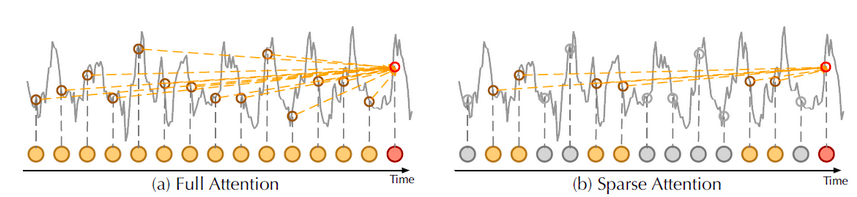
\includegraphics[width=\linewidth]{graphs/Sparse_Attention_Example.png}
    \caption{Vanilla self Attention and Sparse Attention from Informer}
    \label{fig:sparse_attention}
\end{figure}

There is no masking in place since it is not necessary to withhold information from the decoder as none exists in its intended form. The only part that is in the decoders place is an empty vector with the time horizons that are being forecasted. These timestamps are being converted using the same positional encoding as in the embeddings part. Therefor all that is going to happen in the 'decoder' part is the continuation of predicting values for unseen timestamps.

The arcitecture of the transformers utilising the sparse attention mechanism is shown in figure \ref{fig:eFormer_sparse} where both model variants are displayed. The inner workings of both models are the same for the sparse attention, the only difference lies in the application of the attention to both the mean and the variance while the other model only applies to the mean.

\begin{figure}[!ht]
    \hspace*{\fill}
    \begin{subfigure}[b]{0.4\linewidth}
        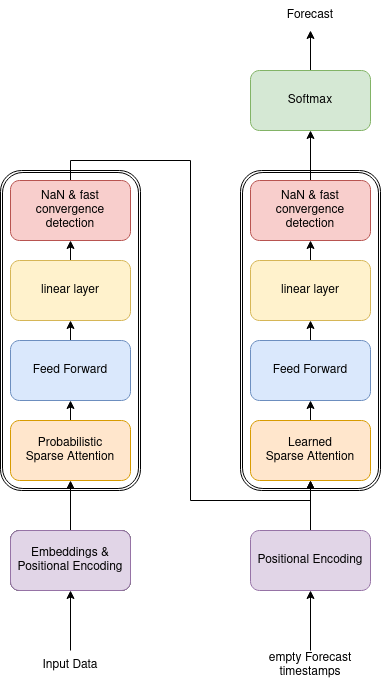
\includegraphics[width=\linewidth]{graphs/eFormer_probSparse.png}
        \caption{probabilistic}        
    \end{subfigure}
    \hfill
    \begin{subfigure}[b]{0.4\linewidth}
        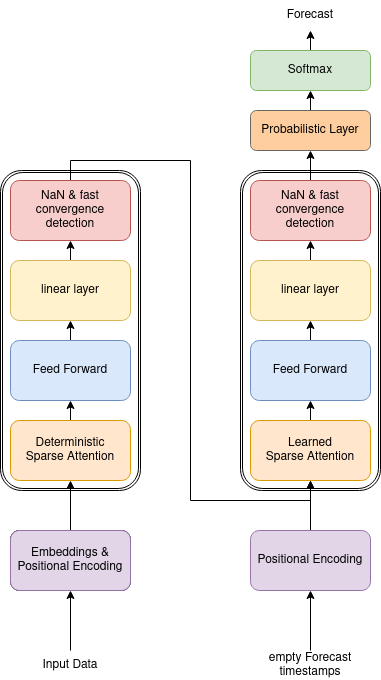
\includegraphics[width=\linewidth]{graphs/eFormer_det_sparse.png}
        \caption{deterministic}
    \end{subfigure}
    \hspace*{\fill}
    \caption{eFormer Sparse Attention}
    \label{fig:eFormer_sparse}
\end{figure}

The key to reduce the computational costs is to build subsets of the key vectors $K$ by sampling for every query vector $Q$. These two vector have the dimensions $[B,H,L_K,D]$ and $[B,H,L_Q,E]$ respectively, with
\begin{itemize}
    \item $B$ as the batch size,
    \item $H$ as the number of multi-attention-heads,
    \item $L_K$ and $L_Q$ as the lengths of the query and key sequences respectively,
    \item $D$ and $E$ as the dimensions of the query and key vectors respectively.
\end{itemize}
This is achieved in the \textit{ProbAttention} class, where at first $U_{part}$ elements are being sampled with
\begin{equation}
    U_{part} = c \ceil*{log(L_K)}
\end{equation}
where $c$ is a hyperparameter, $L_K$ is the length of the key vector that is being sampled and $\ceil*{\cdot}$ is a ceiling function to ensure that $c$ is multiplied with integers as the value for $U_{part}$ can not be fractional. The logarithmic scaling is in place to prevent linear scaling with increased input size, since not every additional element is proportionally as important for the sampling to be effective. After sampling from the original $K$ using the function \textit{torch.randint} the tensor $K_{sample}$ of length $U_{part}$ the dot product is build
\begin{equation}
    QK^{T}_{sample} = Q \cdot K_{sample}
\end{equation}
with the usage of the sampled vector the first step towards reducing the computational load is achieved. This dotproduct is then used in the sparsity measurement to determine which queries have the highest potential impact on the output. This is calculated by
\begin{equation}
    M = max\left(QK^{T}_{sample}\right) - \frac{\sum QK^{T}_{sample}}{L_K}
\end{equation}
of this sparsity measurement the top $n$ values are selected, the number of $n$ is calculated similarly to the $K_{sample}$ using
\begin{equation}
    u = c \ceil*{log(L_Q)}
\end{equation}
where $c$ is the same hyperparameter as before and $L_Q$ is the length of the query vector, the same logic of utilising a logarithm is applied here too. The final step is to calculate the reduced dot product which consists of the selected queries and the full key length
\begin{equation}
    Q_{selected}K^{T} = Q_{selected} \cdot K
\end{equation}
resulting in the the desired lowered computation of $O(T log(T))$ as claimed by \cite{Informer}. \par 

The next step in calculating the attention is to initialize and calculate the attention scores which is performed in the same class as the calculation of the reduced dotproduct. The initial context vectors are the averages over the value tensor $V$ with dimensions $[B,H,L_V,D]$. This can be done since as mentioned previously the masking is not important in this model as the decoder is practically non-existent and thus no future tokens have to be hidden, with the intention to reduce the computational costs further. After the initialised context vectors, they have to be updated. To do so is to use the softmax function on the previously calculated dotproduct to convert them into probabilities, but before that the attention scores are scaled to prevent to large values in the softmax to improve numerical stability. Hence the next steps are
\begin{align}
    a_{ijk} &= a_{ijk} \frac{1}{\sqrt{D}} \\
    a_{ijk} &= \frac{e^{a_{ijk}}}{\sum^{L_K}_{k=1}e^{a_{ijk}}}
\end{align}
where $a_{ijk}$ represents the normalized attention weight for the $k$-th key vector when attending to the $j$-th query in the $i$-th batch for a specific head and $D$ is the dimensionality of the head. The updated context vector is then processed for each selected query index by aggregating information across the value sequence, weighted by the relevance of each value vector as determined by the attention scores.
\begin{equation}
    context_{in}[:,:,index,:] = \sum^{L_K}_{k=1} a_{ijk} \cdot V_{:,:,k,:}
\end{equation}
For the updated context scores the normalized attention scores $a_{ijk}$ are used as weights. \par 

The next class is an Attention Layer that orchestrates all the functions explained before and ensures the correct dimensions for the output tensor and thus builds the core component of the multi-head attention mechanism since this function allows for parallel computing. In detail this class contains 4 steps, where the first one is a linear projection of the query, key and value matrices to bring them to the correct dimensions to ensure computing without problems.
\begin{align}
    Q' &= QW^Q \\
    K' &= KW^K \\
    V' &= VW^V
\end{align}
The weight matrices $W^{Q,K,V}$ come from a linear layer using the weight computations from before. After that the projections are reshaped to make parallel computing across the multi attention heads possible. The second step is the attention computation itself which utilises all the functions described in Detail before. Which results in 
\begin{equation}\label{eq:Encoder-Attention}
    Attention(Q', K', V') = softmax \left( \frac{Q'K'^T}{\sqrt{D / H}} \right) V'
\end{equation}
Here $Q'K'^T$ calculates the dot-product attention scores, while $\sqrt{D/H}$ is the scaling factor that prevents the scores from growing too large as described before.  In the third step the results from the different are combined and mixed to take full advantage of the multi-attention head mechanism as been shown for NLP tasks by \cite{multi-head-mixing, mulit-head-mixing2}. Doing so allows the model to learns from different aspects from the same data and is able to see more perspectives allowing for a richer and more comprehensive representation of the underlying data. Further this allows for better generalization and faster convergence, since each can specialize more and then synergies their results which in turn increases training stability. The final fourth step is another linear projection to bring the Attention from equation \ref{eq:Encoder-Attention} into the desired shape before proceeding. \par 

This concludes the description of the Encoder Model for the Sparse Attention Model, the Decoder part is as stated previously as minimalistic as possible and only consists of an empty vector of positional encoding for the forecasted values and is then put through the same attention mechanism as the encoder part.

The sparse Decoder Part is a customised version of a minimalist transformer decoder that is specialized into working with timer series data and the sparse attention mechanism from the encoder part. It utilises dropout to prevent overfitting and works with the ReLu activation function, while the input to this part is the output tensor from the encoder part and the newly created prositional encodings for the to be predicted values. The forward pass contains deals with positional encoding, cross-attention, a feed-forward network, layer normalization and output generation. While this seems like a lot is done in these steps, several elements have been left out for example the self-attention on the input data purely in the decoder part and the corresponding masking. The only steps that could be omitted is the feed-forward network with its two convolutional layers, except for that the other parts are mandatory in the generation of the forecasts.\par 
The first part the positional encoding used to create the vector of forecasted values utilises the same functions as in the encoder part previously described in equation \ref{eq:pos-encoding} and thus creates a continuation in the time encoding that is easier to understand for the computer. The second part the cross-attention layer takes inputs from the decoder as well as the encoder side and thus is able to combine the relevant data. The Queries $Q$ are the positional encodings from the decoder while the keys $K$ and values $V$ are from the encoder side. These tensors are fed into the same structure as presented in the encoder part in \ref{eq:Encoder-Attention} but with altered inputs hence the equation is now
\begin{equation}\label{eq:Decoder-CrossAttention}
    Attention(Q_{Decoder}, K_{Encoder}, V_{Encoder}) = softmax \left( \frac{Q_{Decoder} K_{Encoder}^T}{\sqrt{D / H}} \right) V_{Encoder}
\end{equation}
as before the keys and values are sampled and thus smaller versions of the original keys and values, as previously described in the encoder part, which again makes the calculation less computational expensive. 
The third part is a feed-forward network which through its non-linear activation function is able to capture more complex patterns in the observed data. The first convolutional layer performs a element-wise transformation using a kernel of size 1 to transform the dimensionality from the inital dimensions set in the hyperparameters $d_{model}$ to the dimension of the feed forward network's hidden layer) $d_{ff}$
\begin{align}\label{eq: decoder-ffn}
    FFN_1 &= ReLu(Conv_{kernelsize = 1}(Attention(Q_{Decoder}, K_{Encoder}, V_{Encoder}))) \\
    FFN_2 &= Conv_{kernelsize = 1}(FFN_1)
\end{align}
to be able to keep working with the attention outputs they are transformed back into the dimensions of $d_{model}$ using a second convolutional layer, without a activation function, since that has already been applied before. The choice for the usage of convolutional layers comes down to the benefits they provide over fully connected dense layers in traditional transformer models, which are mainly the efficiency advantages of sharing parameters and their ability to be easily parallelized, as well as the application of filters on smaller regions due to the kernel size of $1$ which provides benefits to capturing short term dependencies.

The fourth step include layer normalization which ensure the model's stability and help to mitigate the vanishing gradient problem. The normalization is applied towards the normal attention output as well as the feed-forward network output
\begin{align}
    Attention(Q,K,V) &= LayerNorm(Attention(Q,K,V) + Dropout(Attention(Q,K,V)) \\
    FFN_3 &= LayerNorm(Attention(Q,K,V) + Dropout(FFN_2))
\end{align}
with the dropout of $0.1$, some of the neurons in the layers are deactivated to boost generalization of the model by forcing it to find new paths when previous attempts are blocked.
In the last step the tensor from $FFN_3$ is processed into the forecasted values by using a linear layer
\begin{equation}
    forecast = FFN_3 W + b
\end{equation}
with $W, b$ being the weights and biases respectively that are used in the linear layer. After this transformation the forecast is an interpretable value that can be compared to the ground truth and thus the error can be calculated and the back propagation steps can start to update the weights.

\subsubsection{Auto Correlation Attention}

\subsubsection{Loss Function}

As mentioned in the description for the eFormer, a custom Loss function is implemented. The idea is to use a function that works especially well with probabilistic models but can also handle deterministic ones. The choice fell on CRPS which stands for continuous ranked probability score, since it is a more specialised version of the MAE. For deterministic models the CRPS calculates the MAE and thus deterministic and probabilistic models can be compared. In the version that is used here, it is further customised by including the weights after claculating the differences between the predicted and true values, hence some value pairs are having a greater impact on the calculation of the overall score compared to the vanilla CRPS where each value pair has the same significance on the overall loss score. The individual steps to calculate the loss are the following: at first all inputs are reshaped into the same dimensions. This affects the predictions where a singleton dimension is removed and the weights where again a singleton dimension is removed and the average over the last dimension is calculated to have all inputs as a vector of the same length as the sequence length set in the hyperparameters. The CRPS uses a cumulative distribution function (CDF), but to use this function the values in the forecast vector have to be sorted first, after that the cumulative sum of sorted forecasts can be calculated
\begin{equation}
    CDF = \frac{1}{N} \sum^N_{i = 1} \mathcal{I}(f_i < f)
\end{equation}
with $f_i$ being the forecasted values, $N$ the total number forecasts and $\mathcal{I}$ being an indicator function approxamated by the cumulative sum over the forecasts. The indicator function $\mathcal{I}$ compares the forecasted values with the true values
\begin{equation}
    \mathcal{I} (f,t) = \begin{cases}
        1, & f > t \\
        0, & \text{otherwise}
    \end{cases}
\end{equation}
hence the final equation for the CRPS calculation is
\begin{equation}
    CRPS = \frac{1}{N} \sum^N_{i = 1} w_i (CDF_{forecast_i} - \mathcal{I}(f_i,t))^2
\end{equation}
where $w_i$ is the weight matrix from the decoder part that enables the weighted mean, the final score is therefor the weighted mean of all forecasts. The differences towards the theoretical part covered earlier lies in the indicator function where the comparison is towards the true values rather than $0$ and the usage of weights in the final calculation to put more significance on value pairs with higher weights associated.

\subsection{Experiment Setup}

The same models are trained on different parameters, as stated in the beginning the overarching goal is to forecast for different forecast horizons. For the longer forecast horizons the look back window has to be larger to give the chance of capturing more context in the larger pool of data. To check if these larger windows have a general benefit on forecasting the shorter forecast horizons are also tested on the larger look back windows. Therefor the following setups shown in \ref{tab:forecast-lookback} can be derived for each model with different sizes for the embedding vectors. 

\begin{table}[h!]
  \begin{center}
    \begin{tabular}{c|c|c|c|c|c}
      \toprule % <-- Toprule here
       & \multicolumn{5}{c}{\textbf{Look Back Window}} \\
      \textbf{Forecast} & 6h & 12h & 24h & 48h & 72h \\
      \midrule % <-- Midrule here
      10 min & x & x & x & x & x \\
      1h &  & x & x & x & x \\
      6h &  &  & x & x & x \\
      12h &  &  &  & x & x \\
      24h &  &  &  &  & x \\
      \bottomrule % <-- Bottomrule here
    \end{tabular}
    \caption{Combination of Forecast Horizon with Look Back Window Size}
    \label{tab:forecast-lookback}
  \end{center}
\end{table}

All of these combinations are run for different lengths of the embedding vectors, these are namely $[32, 64, 128]$, these values have been chosen since they are all powers to the basis of two and these length are also discussed by \cite{optimal_embedding_length}. A longer embedding length correlates with fewer close matches, since the embeddings paint a more detailed picture with increasing length of the data they describe as shown in \cite{introduction_embeddings}. Therefore the sharpness of the embedding vectors increases but in practice this is not always advisable, since the close equivalents in the n-dimensional space they are compared in has fewer vectors as they spread out more. On the other side if the size for the embedding vector is chosen to small, not enough information and details are stored in the embedding vectors and too many close equivalents exist since the space contains less dimensions where the vectors could spread out to.

Next to the different embedding length', several Loss functions are being implemented and tested to see if they hold any measurable differences for the task at hand. The loss functions in question are:
\begin{multicols}{2}
\begin{itemize}
    \item custom CRPS
    \item MSE Loss
    \item L1 Loss
    \item Cross-Entropy Loss
\end{itemize}    
\end{multicols}
The CRPS and the L1 Loss could present similar results as the L1 Loss utilises the mean absolute error (MAE), on which also the CRPS is build. Hence with a deterministic model with non-learnable variance these two models are resulting in the same loss values. The MSE Loss is being used by \cite{Informer, autoformer} and therefor it is used here again to compare the results under similar conditions. And the Cross-Entropy Loss is used as it finds application in diverse fields including time series analysis as shown by \cite{cross-entropy_time-series}. It is not expected that one loss outperforms the others, especially not in the deterministic cases. Though for the probabilistic cases it is expected that the CRPS loss achieves better results as this function is especially designed for the usage of probabilistic forecasts. 

As previously discussed the models that are used are 
\begin{multicols}{2}
\begin{itemize}
    \item custom eFormer
    \item Vanilla Transformer
    \item Informer
    \item Single Layer Perceptron
\end{itemize}
\end{multicols}
where the Linear Model the Single Layer Perceptron acts as the absolute benchmark to beat, while the Vanilla transformer by \cite{vanilla-transformer} is the general purpose deep learning benchmark, as this model is developed to work primarily with language data and not time series. The other two models are build to work better with time series data, therefore it is expected that both models perform better compared to the other two models in terms of accuracy as well as computational costs compared to the Vanilla Transformer, as they have special Attention Modules that decrease the cost of computation. The fastest and cheapest model to train and use is expected to be the linear model, as it only contains one linear layer.

\section{Results}

The results are stored for each of the aforementioned combinations as different data frames, which are then combined into a dictionary to easily access all the required information filtered by the set parameters. The Results data frames are separated into three distinct groups
\begin{multicols}{3}
    \begin{itemize}
        \item Hardware Usage
        \item Epoch duration \& Loss
        \item Predictions \& Labels
    \end{itemize}
\end{multicols}
From these groups the last one is only intended for a visual presentation since the difference between the included time series is already calculated in the Validation Loss, which in turn is part of another group.

The results of the hardware usage are measured every ten seconds for the CPU, RAM and GPU, therefore this is a good approximation how much maximum and average capacity the system needs for the duration of the training process. The step of measuring every ten seconds has been chosen to capture events of spikes, which in the first runs have lasted for more than ten seconds, but not less than ten seconds to limit the constraint this parallel process puts on the system and to keep the resulting data frame at reasonable sizes. 

The final group the epoch duration and loss data frames capture as the name suggests the duration of one iteration of training and validation process and the validation loss calculated at the end of one such iteration. These data points are used to further enhance the estimation of the effectiveness of the models, for the duration this acts as relevant variable for the efficiency in terms of computational costs, since most services such as AWS and Lambda base their price on the time one is using their machines. On the other hand the validation loss is an indicator how effective a model is at making good predictions compared to other models and while observing the change in the validation loss, one can see how fast or slow the models converge to their final points and when they have reached their lowest point as they hit the early stopping limit. The fast convergence is a good sign as this signals that the models are potentially finishing their training faster than other models, and thus also save resources.

\subsection{Hardware Usage}

For the Hardware Decision it is most useful to know the maximum values one training process can reach, as this is one of the determent factors to decide which hardware specifications to use. The other variable that is regarded as relevant is the average usage, as this can help to estimate the power consumption of the servers or computers used.

\begin{table}
    \centering
    \begin{tabular}{l|c|S|S}
        \toprule
        \textbf{Loss Function} & \textbf{Embedding Length} & \textbf{max Usage} & \textbf{avg Usage} \\
        \midrule
        CRPS & 64 &  &  \\
        MSE  & 64 &  &  \\
        L1   & 64 &  &  \\
        Cross Entropy & 64 &  &  \\
        \bottomrule
    \end{tabular}
    \caption{Linear Model Results}
    \label{tab:linear_results}
\end{table}

\subsection{Epoch Duration \& Loss}

\subsection{Predictions vs Labels}

\newpage

\printbibliography

\end{document}